\documentclass{article}
\usepackage[utf8]{inputenc}
\usepackage[margin=0.7in]{geometry}
\usepackage[colorlinks=true, linkcolor=black, citecolor=black]{hyperref}

\usepackage[english]{babel}
\usepackage{graphicx}
\usepackage{subcaption}
\usepackage{caption}
\usepackage{amsmath, amssymb, bm}

\usepackage[backend=biber]{biblatex}
\usepackage{array}
\usepackage{xcolor}
\usepackage[ruled,vlined,noline]{algorithm2e}
\usepackage{epsfig}
\usepackage{hyperref} 
\usepackage{cleveref}
\usepackage{glossaries}

\usepackage{makecell}
\usepackage{tikz}
\usepackage{microtype}
\usepackage{float}

\usepackage{listings}
\usepackage{xcolor}


% Define colors for GitHub dark mode appearance
\definecolor{background}{rgb}{1, 1, 1}
\definecolor{comment}{rgb}{0.5, 0.5, 0.5}
\definecolor{keyword}{rgb}{0.13, 0.54, 0.13}
\definecolor{identifier}{rgb}{0, 0, 0}
\definecolor{string}{rgb}{0.63, 0.13, 0.94}
\definecolor{function}{rgb}{0.18, 0.18, 0.78}
\definecolor{number}{rgb}{0.56, 0.35, 0}
\definecolor{rulecolor}{rgb}{0.8, 0.8, 0.8}

% Configure the listings package
\lstset{
    backgroundcolor=\color{background},
    frame=single,
    rulecolor=\color{rulecolor},
    frameround=tttt,
    basicstyle=\ttfamily\footnotesize\color{identifier},
    keywordstyle=\color{keyword}\bfseries,
    identifierstyle=\color{identifier},
    commentstyle=\color{comment}\itshape,
    stringstyle=\color{string},
    numberstyle=\tiny\color{rulecolor},
    stepnumber=1,
    numbersep=10pt,
    showstringspaces=false,
    breaklines=true,
    tabsize=4,
    captionpos=b,
    language=Python,
    morekeywords={self, np, plt, def, sample, plate, partial, jax},
    literate=*{:}{{\textcolor{number}{:}}}1
             {=}{{\textcolor{number}{=}}}1
             {+}{{\textcolor{number}{+}}}1
             {-}{{\textcolor{number}{-}}}1
             {*}{{\textcolor{number}{*}}}1
             {/}{{\textcolor{number}{/}}}1
             {>}{{\textcolor{number}{>}}}1
             {<}{{\textcolor{number}{<}}}1
             {,}{{\textcolor{number}{,}}}1
             {(}{{\textcolor{number}{(}}}1
             {)}{{\textcolor{number}{)}}}1
             {[}{{\textcolor{number}{[}}}1
             {]}{{\textcolor{number}{]}}}1
}

% Define a custom function style
\lstdefinestyle{mystyle}{
    morekeywords=[2]{somefunction}, % Add your function names here
    keywordstyle=[2]{\color{function}}
}

% Apply the custom style
\lstset{style=mystyle}


\addbibresource{report/library.bib}


\newcommand{\Norm}{\mathcal{N}}
\newcommand{\argmax}{\text{argmax}}
\newcommand{\nt}{$n_\text{train}$}

\newcommand{\bacc}{ Fortgeschrittene Programmierung \\ in der Physik SE}

\begin{document}

\begin{titlepage}
    \begin{figure}
    %
\includegraphics[width=2.cm]{logo-itp.png} \hfill
    %\includegraphics[width=2.5cm]{logo_tug_en.jpg} \par
    
\includegraphics[width=3.cm]{logo-itp.png} \hfill
    
\includegraphics[width=3.5cm]{logo-tu.png} \par
    %\hrulefill
    \end{figure}
    
    \begin{center}
    {\huge\sc \bacc} \\ Institute of Theoretical Physics\\
    Computational Physics\\
    
    \vspace{5cm}
    {\huge\sc Introduction to Baysian Neural Networks with examples in Physics and Engineering} \par
    Advisor: \\ Univ.-Prof. Dipl.-Phys. Dr. Wolfgang von der Linden \\ 
    \vspace{5cm}
    
    {\Large\sc Tobias Leitgeb}
    
    {Mat.Nr. 12006992}
    
    \vspace{3cm}
    Summer term 2024
    \end{center}
    \end{titlepage}
\section{Introduction}
In this report we will look at the basics of Baysian Neural Networks, how to implement them and at some specific exemplary problems. Additionally, there will be a short introduction to Baysian PINNs \cite{Yang_2021}. I want to give a quick overview of the mathematics needed for defining a Baysian Neural Network, training it and predicting new samples. For implementing the BNN, \textit{NumPyro} \cite{bingham2019pyro, phan2019composable} is used, which is a probabilistic library build in \textit{JAX} \cite{jax2018github}. This \textit{JAX} backend provides very fast and efficient computing through access to JIT compilation, automatic differentiation and support of CUDA. Through some examples, the basic of \textit{NumPyro} and \textit{JAX} will be shown. The complete code used in this report can be found at \href{https://github.com/TobiLeitgeb/BNN_project}{my github}.
\section{Mathematical basics}
\subsection{Baysian Neural Networks}
A Baysian Neural Network is a Neural Network with stochastic features, like probability distributions for the weights or for the activation functions \cite{BNNTut}. For training general Neural Networks, one maximizes the likelihood $p(\mathcal{D}|\bm \theta)$ to obtain a point estimate $\bm \theta^*$:
\begin{equation}
    \bm \theta^* = \argmax_{\bm{\theta}} p(\mathcal{D}|\bm \theta)
\end{equation}
The training of the BNN on the other hand, is done by calculating the posterior distribution of the parameters $p(\bm \theta | \mathcal{D}$), given the training data $\mathcal D$. This posterior is given by Bayes rule:
\begin{equation} \label{eq:post_params}
    p(\bm \theta|\mathcal{D}) = \frac{p(\mathcal{D}|\bm \theta)p(\bm \theta)}{\int_{\theta'}p(\mathcal{D}|\bm \theta')p(\bm \theta')}
\end{equation}
with the likelihood $p(\mathcal{D}|\bm \theta)$, the prior for the parameters $p(\bm \theta)$ and the integral for the evidence $\int_{\theta'}p(\mathcal{D}|\bm \theta')p(\bm \theta')$. This integral over all possible parametrizations of the Network is, most of the time, intractable due to its high dimensionality, which is especially true for deep Neural Networks. Therefore, we need to somehow approximate this posterior distribution. There are several methods for doing inference, e.g \textit{Monte Carlo dropout, Markov Chain Monte Carlo, Laplace approximation, Variational Inference, Deep ensembles} etc. \cite{murphy}. In this report, the focus will be on two inference methods, which are arguably the most robust and widely used algorithms for BNNs \cite{BNNTut}:
\begin{itemize}
    \item Markov Chain Monte Carlo
    \item Variational Inference
\end{itemize}
\subsection{Markov Chain Monte Carlo}
A very strong quality of \textit{MCMC} methods is that they do not restrict or assume the form of the posterior, which we will later see, has to be done when using variational methods. \textit{MCMC} is especially a good choice, when the Network is rather thin with a small number of neurons and layers. This is because \textit{MCMC} does not scale that well when the dimension of the parameters greatly increases. However, efforts have been made for adapting \textit{MCMC} for bigger BNNs \cite{murphy}. Later on, this behaviour will be shown by specific examples. Another drawback is that the whole training set has to be used, and therefore kept in memory, for every training step. This further limits the capabilities for big datasets and deep Networks.\\
\textit{NumPyro} allows a very simple and clear syntax for defining and doing inference with \textit{MCMC}. In this example we use the so called NUTS algorithm, which is a variant of Hamilton Monte Carlo \cite{Brooks_2011, hoffman2011nouturnsampleradaptivelysetting}.
\begin{lstlisting}[caption= {Inference with NUTS},captionpos=t]
from numpyro.infer import NUTS, MCMC
#define pseudo random number generator key
inf_key = jax.random.PRNGKey(0)
#define mcmc with the NUTS sampler, the network and the number of samples
mcmc = MCMC(NUTS(BNN_model), num_warmup=1000, num_samples=1000)
#running inference with the training data 
mcmc.run(inf_key, X_train, Y_train, LAYERS)
mcmc.print_summary()
\end{lstlisting}
After running the inference, the summary gives an overview of the calculated samples for the parameters of the network:
\begin{lstlisting}[caption= {Results of Inference with HMC},captionpos=t]
sample: 100%|██████████| 2000/2000 [04:36<00:00,  7.23it/s, 1023 steps of size 6.49e-04. acc. prob=0.93]

                             mean       std    median      5.0%     95.0%     n_eff     r_hat
                W0[0,0]     -0.06      0.98      0.06     -1.71      1.31     12.27      1.10
                W0[0,1]     -0.14      0.82     -0.11     -1.71      1.05     33.64      1.10
                W0[0,2]     -0.03      0.84     -0.09     -1.29      1.37     25.33      1.21
                W0[0,3]     -0.04      0.92     -0.03     -1.66      1.33     15.52      1.10
                W0[0,4]     -0.24      0.72     -0.22     -1.44      0.90     27.59      1.06
                W0[0,5]      0.12      0.95      0.10     -1.46      1.72     40.72      1.06
                W0[0,6]      0.14      0.67      0.10     -0.96      1.27     61.09      1.00
                W0[0,7]      0.22      0.95      0.13     -1.22      1.88     25.26      1.01
                W0[0,8]     -0.17      0.89     -0.15     -1.70      1.17     29.00      1.03
                W0[0,9]     -0.05      0.79     -0.03     -1.42      1.24     38.40      1.05
               W0[0,10]      0.06      0.86      0.04     -1.46      1.43     13.57      1.13
               W0[0,11]      0.20      0.88      0.23     -1.10      1.85     30.89      1.05
               W0[0,12]      0.16      0.87      0.23     -1.37      1.62     32.36      1.12
               W0[0,13]      0.03      0.95     -0.05     -1.56      1.59     24.91      1.00
...
                  b2[0]      0.26      0.94      0.29     -1.18      1.81     34.99      1.01
  observation precision     44.33      6.95     44.19     34.01     56.20     14.91      1.08

Number of divergences: 2
\end{lstlisting}

\subsection{Variational Inference}
In variational inference the idea is to approximate the posterior distribution with a parameterized approximated distribution $q_\phi (\bm \theta)$. The parameters $\phi$ of this distribution are now optimized, such that they best describe the posterior. For this the Kullback-Liebler divergence is used as a measure of similarity between two probability distributions $p$ and $q$ \cite{murphy, BNNdistill}:
\begin{equation}\label{eq:kullback}
    d_{KL} [q(\bm \theta)|| p(\theta|\mathcal{D})] &= \int_{\bm \theta'} q_\phi(\bm \theta) \log \frac{q_\phi(\bm \theta)}{p(\bm \theta|\mathcal{D})} d\bm \theta\\
    &=\mathbb{E}_{q_\phi(\bm \theta)}[\log(q_\phi(\bm \theta) - \log p(\bm \theta|\mathcal{D})]
\end{equation}
The optimization problem can then be formulated as \cite{murphy}:
\begin{equation}\label{eq:optprob}
    q = \arg \min_q d_{KL} [q(\bm \theta)|| p(\theta|\mathcal{D}]
\end{equation}
By this optimization, we can obtain the parameters $\phi$ of the variational distribution
For solving this optimization problem, \eqref{eq:kullback} has to be rewritten, since the posterior cannot be directly computed. 
\begin{align}
    \phi &= \arg \min_\phi d_{KL} [q(\bm \theta)|| p(\theta|\mathcal{D}]\nunumber\\
    &= \arg \min_\phi \mathbb{E}_{q_\phi(\bm \theta}[\log q_\phi(\bm \theta) - \log p(\bm \theta|\mathcal{D})]\nonumber\\
    &= \arg \max_\phi \underbrace{\mathbb{E}_{q_\phi(\bm \theta}[\log p(\bm \theta, \mathcal{D}) - \log q_\phi(\bm \theta)]}_{\Tilde{\mathcal{L}}(\phi) = \text{ELBO}} + \log p(\mathcal{D)}\\
\end{align}
where the marginal data likelihood $p(\mathcal{D})$ can be left out for the optimization of $\phi$, since it does not depend on the variational parameters. Here the evidence lower bound (ELBO) is introduced. The name of the ELBO comes from the fact that it is the lower bound of the evidence $p(\mathcal{D})$, s.t. \cite{murphy}:
\begin{equation}
    \Tilde{\mathcal{L}}(\phi) = \mathbb{E}_{q_\phi(\bm \theta}[\log p(\bm \theta, \mathcal{D}) - \log q_\phi(\bm \theta)] \leq p(\mathcal{D})
\end{equation}
With this reformulation, the optimization of the variational parameters is reformulated as the maximization of the ELBO $\Tilde{\mathcal{L}}$ with respect to $\phi$. For actually doing this optimization, there are several methods. One of the most popular is \textit{Stochasitc Variationl inference} \cite{hoffman2013stochasticvariationalinference}. SVI generally works just like stochastic gradient ascent \cite{BNNTut} and comes with advantages like minibatching. Other methods are \textit{Bayes by backpropagation}, \textit{Laplace approximation} or \textit{Deep ensembles}.\\
At last, we briefly want to demonstrate how to do VI in \textit{NumPyro}:
\begin{lstlisting}[caption= {Inference with VI},captionpos=t]
from numpyro.infer.autoguide import AutoDiagonalNormal, AutoLaplaceApproximation, AutoMultivariateNormal, AutoIAFNormal, AutoLowRankMultivariateNormal, AutoDelta
#define the 
guide = AutoDiagonalNormal(BNN_model)

svi = SVI(
    wideband_dnn, guide, numpyro.optim.Adam(0.05), Trace_ELBO()
)

svi_result = svi.run(
    jax.random.PRNGKey(0),
    num_steps=3000,
    X=X_train,
    Y=Y_train,
    layers=LAYERS
)
\end{lstlisting}
\subsection{Predictive distribution}
After having obtained samples, or a variational approximation of the posterior $p(\bm \theta|\mathcal{D})$, predictions at unseen test points $\bm x_*$ can be made. For this we have to formulate a distribution $p(f(\bm x_*|\mathcal{D})$, which is obtained by marginalization of the calculated parameters $\bm \theta$:
\begin{equation}\label{eq:predictivedist}
    p(\bm f( \bm x_*) |\mathcal{D}) = \int_{\bm \theta} p(\bm f ({\bm x_*})|\bm \theta ) p(\bm \theta | \mathcal{D})d \bm \theta = \mathbb{E}_{p(\theta|\mathcal{D})} \left[ p(\bm f ({\bm x_*})|\bm \theta )\right]
\end{equation}
Writing the integral in terms of an conditional expectation of the posterior distribution of $\bm \theta$, gives an interesting view of the marginalized distribution, as the exptectation value of a single neural net output wheighted by the posterior ditribution of the parameters given the training data. In \cite{blundell2015weightuncertaintyneuralnetworks} this is described as an \textit{infinite ensenmble} of Neural Networks. In practice we can not calculate an infinite number of networks. However when having obtained enough iid. samples (monte carlo samples) of the posterior distribution $p(\bm \theta|\mathcal{D})$, the expectation value in \eqref{eq:predictivedist} can be approximated. Generating samples of the posterior is slightly different for the two inference algorithms discussed above. When using MCMC, ($\approx$ independent) samples of the posterior are obtained directly. For every sample $\bm \theta_i$, which is a set of parameters, the networks output $p(\bm f(\bm x_*)|\bm \theta_i)$ is computed. We now approximate the expectation value by taking the mean over all the samples. When using VI the process is nearly the same. After having obtained the trained variational distribution $q$, we can sample from that distribution and again do the same thing as described above with the samples. 
\subsection{Physics informed Baysian Neural Network}
In this section, the baysian equivalence of a PINN, a so called B-PINN \cite{Yang_2021}, is quickly introduced and later on used for a simple example. \\
For PINNs the loss function $\mathcal{L}$ is augmented with an additional physics term:
\begin{equation}
    \mathcal{L}(\bm \theta) = \mathcal{L}_{data} + \mathcal{L}_{physics}
\end{equation}
This physics loss is oftentimes defined through a differential equation:
\begin{equation}
    \mathcal{P}_\phi u(\bm x) = f(\bm x)
\end{equation}
with $\mathcal{P}_\phi$ being a parametric differential operator with parameters $\phi$, $u$ the solution of the differential equation and $f$ the forcing term. Lets assume that we have a data set $\mathcal{D}$ consisting of noisy observations of both $u$ and $f$ $\{(\bm{x_u});\bm{y_u}\}$ and $\{(\bm{x_f});\bm{y_f}\}$ with $\bm{y_i} = u(\bm{x_i}) + \mathcal{N}(\bm{0}|\sigma_{ni}^2 I) ; \; i = u,f$. The solution term $u$ is now parameterized with a Neural Network $\Tilde{u}$:
\begin{equation}
    \mathcal{P}_\phi \Tilde{u}(\bm x; \bm \theta) = f(\bm x)
\end{equation}
Since we are working with libraries that have access to automatic differentiation, the derivative of $\Tilde{u}$, and therefore the forcing term $f$ can be calculated directly:
\begin{equation}
    \Tilde{f}(\bm x;\bm \theta, \phi) = \mathcal{P}_\phi \Tilde{u}(\bm x; \bm \theta))
\end{equation}
with $ \Tilde{f}$ as the 
Since we have observations for both the $u$ and $f$ we can calculate the residuals for both, which leads to our two loss terms:
\begin{equation}
    \mathcal{L}(\bm \theta) = \mathcal{L}_{data}(\Tilde{u}; \bm \theta) + \lambda \mathcal{L}_{physics}(\Tilde{f}(\theta))
\end{equation}
were $\mathcal{L}$ would e.g be the MSE.
\begin{lstlisting}[caption= {Physics Informed Neural Net},captionpos=t]
def physics_forward(
        W: List[jax.Array],
        b: List[jax.Array],
        X: jax.Array,
        activation: Callable,
):
    #input layer
    u = partial(forward, W, b, activation=activation)
    u_prime = jax.grad(u)
    u_double_prime = jax.grad(u_prime)

    #vectorize the functions
    u_prime = jax.vmap(u_prime)(X)
    u_double_prime = jax.vmap(lambda x: u_double_prime(x.squeeze()))(X)
    return u_prime, u_double_prime[:, None]
\end{lstlisting}
\\
To formulate this in terms of baysian NN, the posterior is augmented with the additional likelihood for the function $f$:
\begin{equation} \label{eq:post_params_BPINN}
    p(\bm \theta, \phi|\mathcal{D}_u, \mathcal{D}_f) = \frac{p(\mathcal{D}_u, \mathcal{D}_f|\bm \theta, \phi)p(\bm \theta)p(\phi)}{\int_{\theta'}p(\mathcal{D}_u, \mathcal{D}_f|\bm \theta')p(\bm \theta')}
\end{equation}
with the prior distribution for the parameters of the differential equation. If the parameters $\phi$ are a-priori unknown, they can be assigned a prior function $p(\phi)$ and then be learned directly through inference \cite{raissi2017physicsIDL, Yang_2021}.
The joint likelihood can be implemented in \textit{NumPyro} as:
\begin{lstlisting}[caption={Joint likelihood for B-PINN},captionpos=t]
z = forward(W, b, X_u, activation)[:, None]
dz, ddz = physics_forward(W, b, X_f, activation)
f = m * ddz + gamma * dz + k * z

#joint likelihood
numpyro.sample(
    r"Y_u", 
    dist.Normal(z, sigma_obs_u).to_event(1), 
    obs=Y_u
)
numpyro.sample(
    r"Y_f", 
    dist.Normal(f, sigma_obs_f).to_event(1), 
    obs=Y_f
)
\end{lstlisting} 
\section{Setting up the model}
A very default prior for the parameters of the BNN which has proven to work relatively well \cite{BNNTut} is:
\begin{align}
    \bm W \thicksim \mathcal{N}(\bm 0,\bm I)\\
    \bm b \thicksim \mathcal{N}(\bm 0, \bm I)
\end{align}
where we just use two normal distributions as priors for the wheigts and biases. In the used probabilistic framework NumPyro we can define the priors the following way:
\begin{lstlisting}[caption= {Setting up priors for wheits},captionpos=t]
    W = numpyro.sample(f"W{i}", dist.Normal(0, 1).expand(n_in, n_out))
    b = numpyro.sample(f"b{i}", dist.Normal(0, 1).expand((n_out, )))
\end{lstlisting}
Generally, other priors can also be used, however the normal distributions lead to good results. Two  other ways of initializing the weights are e.g Xavier initialization $\alpha_l^2 = \tfrac{2}{n_{in}+n_{out}}$ or LeCun initialization $\alpha_l^2 = \tfrac{1}{n_{in}}$ \cite{murphy}. The weights would then be initialized according to:
\begin{equation}
    \bm W_l \thicksim \Norm(\bm 0, \alpha_l^2 \bm I); \; \bm b_l \thicksim \Norm(\bm 0, \alpha_l^2 \bm I)
\end{equation}
Here $\bm W_i$ and $\bm b_i$ are the corresponding parameters for the i-th layer. Another very important step is to normalize the data:
\begin{equation}
     y_{i, \text{normalized}} = \frac{ y_i - \mu_{\bm Y}}{\sigma_{\bm Y}}
\end{equation}
since there was very poor performance without the normalization. This is necessary, since the priors of the weights are centered around 0 with a variance of 1. Without normalizing the data, one could run into problems getting valid results. For making predictions after training, the values are transformed back:
\begin{equation}
    \hat{y}_i = \hat{y}_{i,\text{normalized}} \cdot {\sigma_{\bm Y}} + \mu_{\bm Y}
\end{equation}
For the feed-forward BNN we can also define a forward pass, which can be written as:
\begin{equation}
    \bm f(\bm x|\bm \theta) = \sum_i w^{(L)}_{ji} \left( \ldots \phi \left( \sum_k w^{(1)}_{mk}x_k + \bm b^{(1)} \right) \right) + \bm b^{(L)}
\end{equation}
After having obtained the samples through inference, the forward pass is the same as for a standard feed-forward neural networks
In \textit{JAX} this can be implemented as:
\begin{lstlisting}[caption= {Feed forward Neural Network},captionpos=t]
def forward(
        W: List[jax.Array],
        b: List[jax.Array],
        X: jax.Array,
        activation: Callable,
):
    #input layer
    z = activation(jnp.dot(X, W[0]) + b[0])

    #hidden layers
    for i in range(1, len(W) - 1):
        z = activation(jnp.dot(z, W[i]) + b[i])

    #output layer with no activation
    z = jnp.dot(z, W[-1]) + b[-1]
    return z.squeeze()
\end{lstlisting} 
With this forward pass and the priors for the parameters $\theta$, the whole model can be set up as a relativly easy function:
\begin{lstlisting}[caption={NumPyro model for baysian deep neural network},captionpos=t]
def BNN_model(
        X: jax.Array,
        Y: jax.Array,
        layers: List[int],
):
    N, input_dim = X.shape
    activation = jax.nn.relu
    W = []
    b = []
    #build the layers with the given list
    for i, layer in enumerate(layers):
        W_, b_ = dense_layer(i, [input_dim, layer])
        W.append(W_)
        b.append(b_)
        input_dim = layer
    #forward pass through the network
    z = forward(W, b, X, activation)
    
    precision_obs = numpyro.sample(r"observation precision", dist.Gamma(3., 1.))
    sigma_obs = 1.0 / jnp.sqrt(precision_obs)

    with numpyro.plate("data", N):
        numpyro.sample(
            "Y", 
            dist.Normal(z, sigma_obs).to_event(1), 
            obs=Y
        )
\end{lstlisting}
When using Variational inference for the inference of the posterior of the parameters, there are no direct samples for parameters. Therefore, the trained variational distribution $q$ (called guide here) has to be used to sample $\bm \theta$:
For predicting new values at $\bm x_*$, we draw samples from the trained variational distribution $q_\theta $
\begin{lstlisting}[caption={Prediction of new samples with VI},captionpos=t]
def predict_new(
        svi_result,
        guide,
        X_test: jax.Array,
        num_samples: int = 500,
        *,
        key: jr.key,
        return_mean: bool = True,
    )-> Tuple:
    
    sample_key, prediction_key = jr.split(key, 2)
    #sample from the trained guide q_phi(theta)
    samples = guide.sample_posterior(
        sample_key, svi_result.params, sample_shape=(num_samples, )
    )
    #define predictive distribution with samples and the model.
    predictive_distribution = Predictive(
        BNN_model, samples, return_sites=["Y"]
    )
    #sample from the predictive distribution given new test points
    predictions = predictive_distribution(
        prediction_key, X_test, None, LAYERS
    )
    if return_mean is True:
        return jnp.mean(predictions["Y"], axis=0), jnp.var(predictions["Y"], axis=0)
    else:
        return jnp.mean(predictions["Y"], axis=0), jnp.var(predictions["Y"], axis=0), predictions
\end{lstlisting}

\section{Numerical examples}
The error functions to quantify the testing error are the relative L2 error and the Normalized Root Mean Squared Error (NRMSE):
\begin{align}
     rel \; L^2 = \sqrt{\frac{\sum_i (\hat{y}_i - y)^2}{\sum_i (y_i)^2}}\\
    \text{NRMSE} = \sqrt \tfrac{1}{n}\sum_{i=1}^n (\hat{y}_i - y)^2
\end{align}
\subsection{Transistor surrogate model/Transformer model akash}
Here the data set consists of an inputs $ \bm x$, which specify the circuit layout and of the envelope of the fourier transformed output of the simulation data $\bm y$ over a specified frequency range.
\begin{align}
    X = \begin{bmatrix}
        \bm x_1^T, \\
        \bm x_2^T\\
        \vdots\\
        \bm x_N^T
        \end{bmatrix} \;, \;
    Y = \begin{bmatrix}
        \bm y_1^T\\
        \bm y_2^T\\
        \vdots\\
        \bm y_N^T
    \end{bmatrix}
\end{align}
with $\bm x_i \in \mathbb{R}^d$ and $\bm y_i \in \mathbb{R}^{p}$. The vector $\bm x_i$ is the design vector for the circuit, with the parameters which are beeing adapted. For this example we have:
\begin{equation}
    x_i = [...]
\end{equation}Therefore, we get two matrices $\bm X, \bm Y$ with shapes $(N, d)$ and $(N, p)$, where $N$ is the number of training points, $d$ is the dimensionality of the input and $p$ is the number of frequency outputs. The BNN is designed as: $\bm f(\bm x, \bm \theta): \mathbb{R}^d \rightarrow \mathbb{R}^p$ to yield an output for the whole frequency range. It would also be possible to use the frequency as a part of the input $\bm x$. However, this would highly increase the complexity of the input space and would not yield better results. In this application the goal is to define a surrogate model for the transformer LT spice model. For this example 500 configurations were simulated. For training we used 200 samples. BNNs are interesting for surrogate modelling, since they also give an uncertainty quantification. When looking at the samples and at the calculated predictions, it is interesting to see that the model quantifies the uncertainty somewhat wrong especially in the are from $10^6 - 10^7 $Hz. Between different circuit parameterizations, there is nearly no difference in these regions. 
\begin{figure}[htbp!]
    \centering
    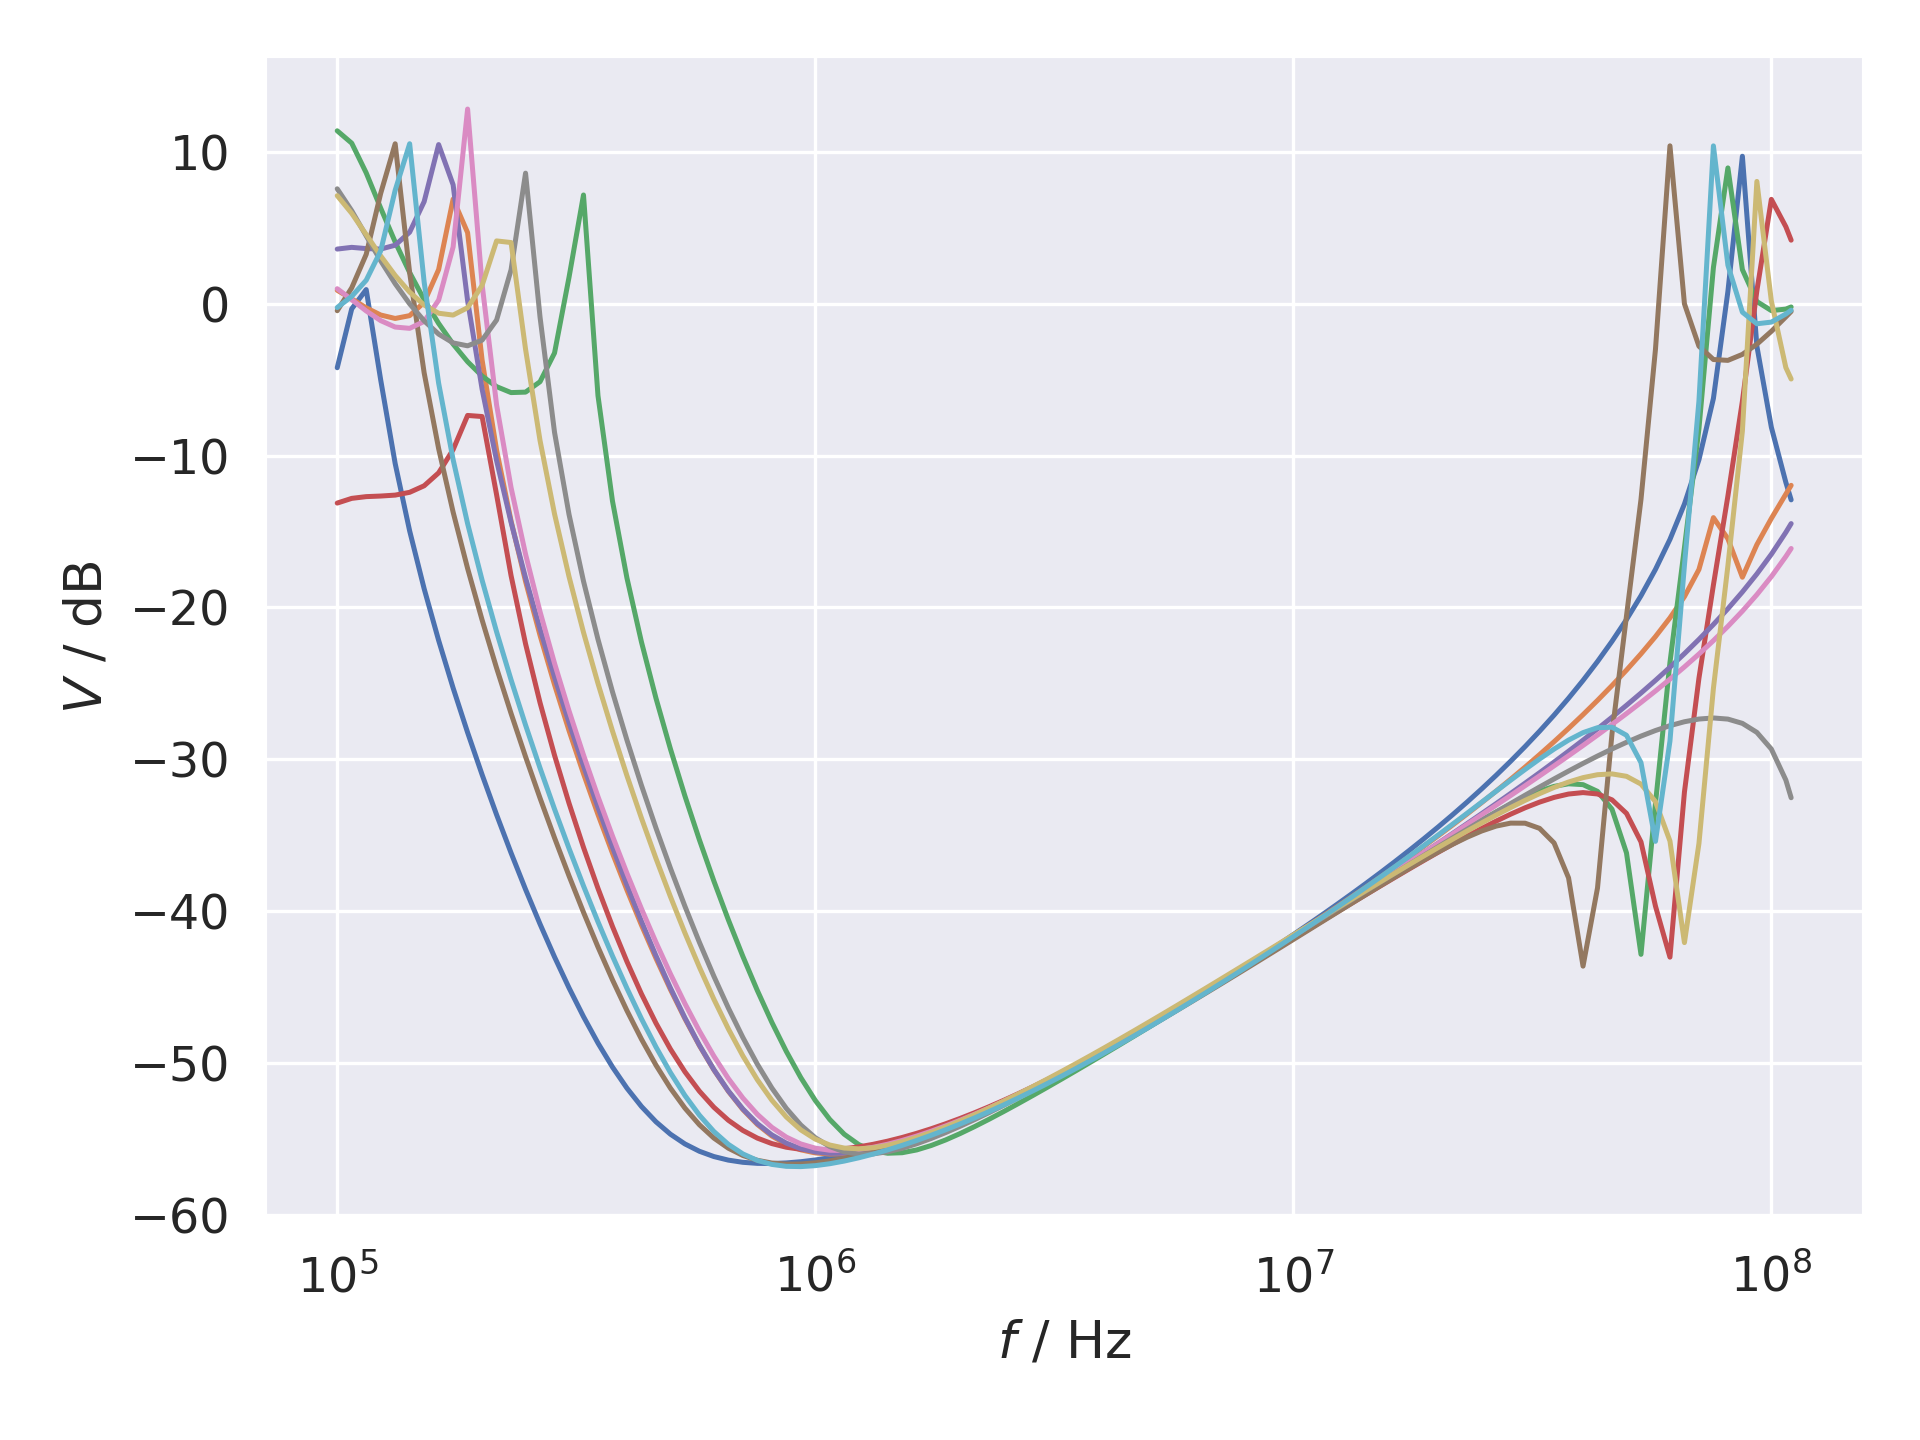
\includegraphics[width=0.6\textwidth]{plots/data_samples.png}
    \caption{Training samples $\bm Y_i$ plotted over the frequency domain. One line is the frequency response for a circuit parameterized by the respective $\bm X_i$.}
    \label{fig:training_samples}
\end{figure}
\begin{figure}[htbp!]
    \centering
    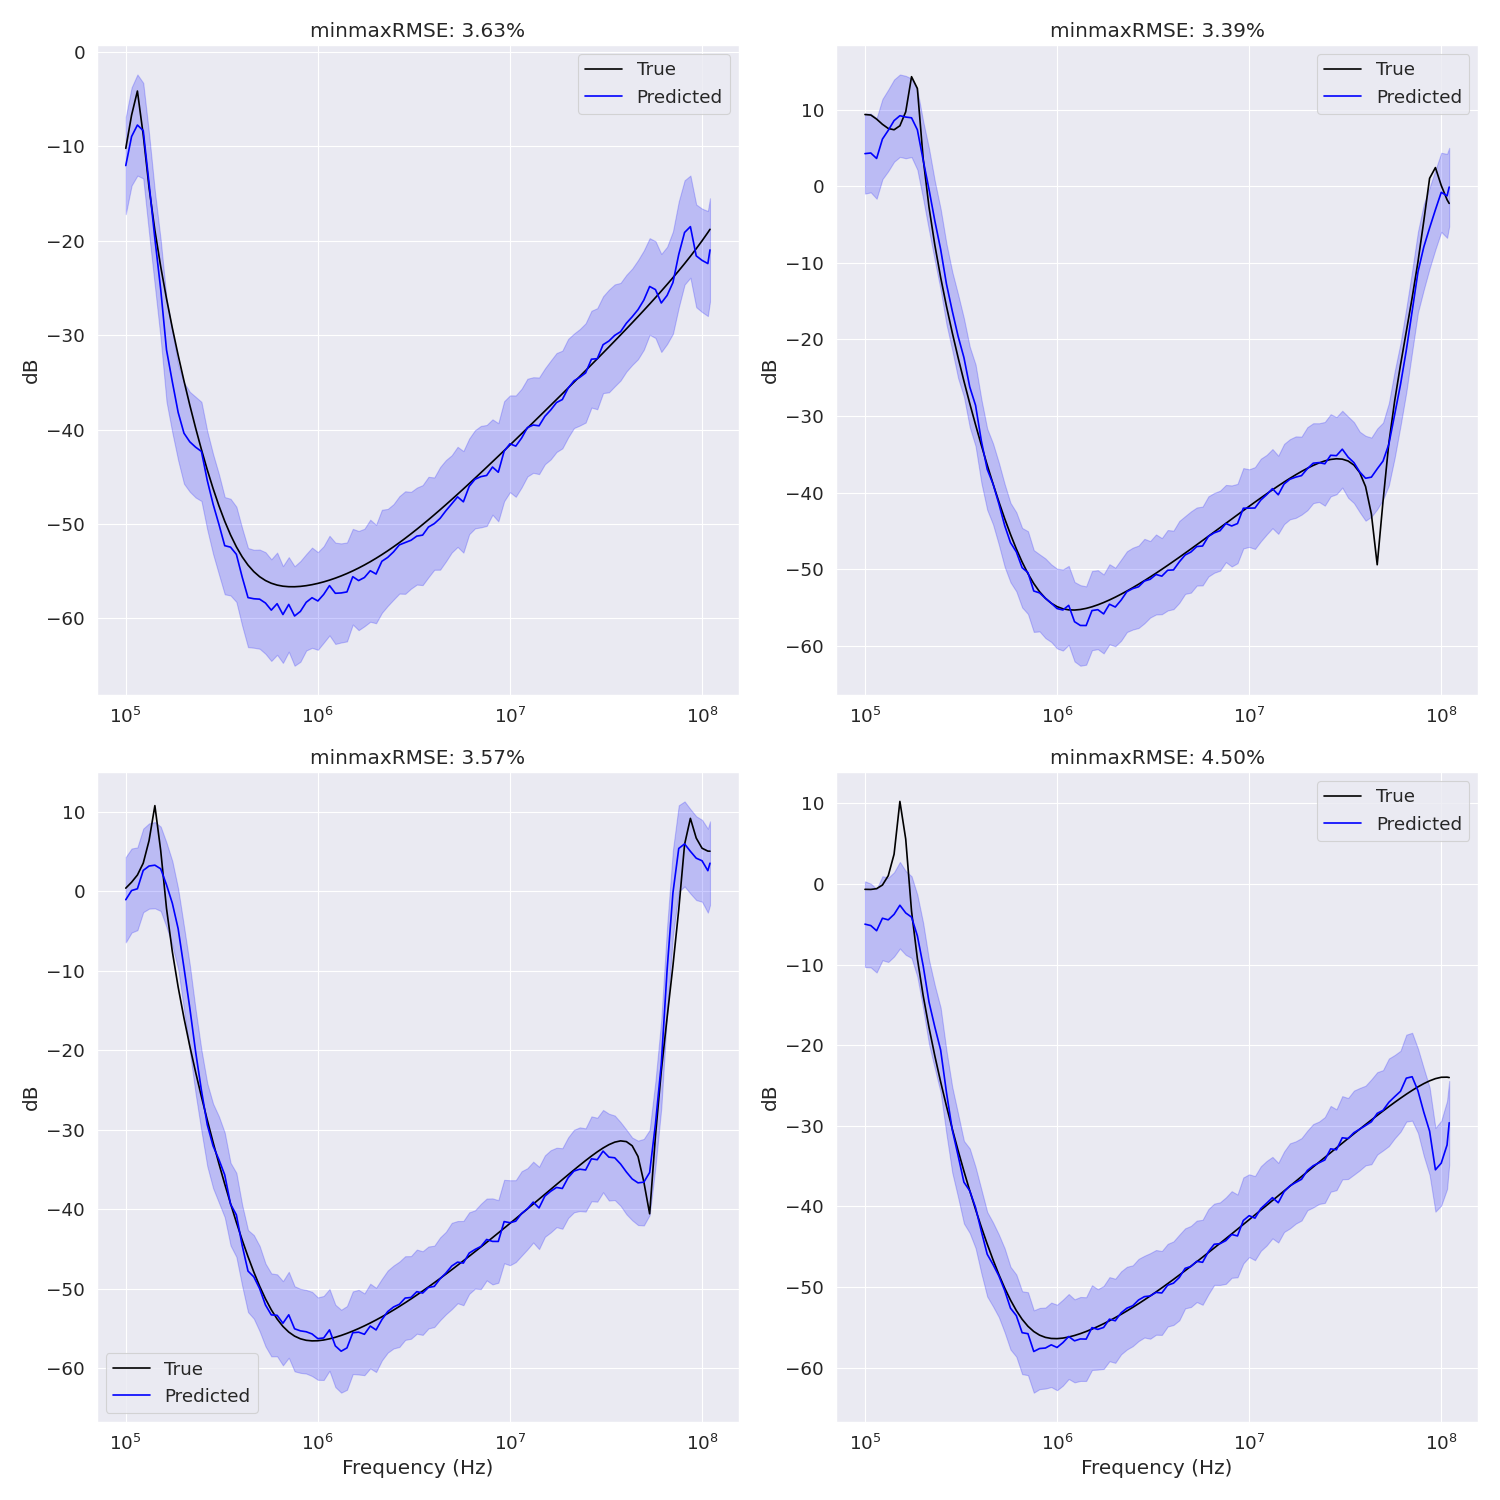
\includegraphics[width=0.6\textwidth]{plots/prediction_transformer.png}
    \caption{Calculated posteriors for test samples $\bm X_\text{test}$. With mean function and 95 \% confidence interval.}
    \label{fig:training_samples}
\end{figure}
\subsection{Damped Oscillator}
Let's consider a one-dimensional differential equation that models a damped oscillator, characterized by a mass $ m $, damping coefficient $ \gamma $, force constant $k$, and initial conditions. The equation governing the system is:

\begin{align}
    & m\frac{\partial^2 u(t)}{\partial t^2} + \gamma \frac{\partial u(t)}{\partial t} + k u(t) = f(t), \\
    & u(0) = 0, \quad \frac{\partial u(t)}{\partial t}\bigg|_{t=0} = 0
\end{align}
The specific case we're examining uses the parameters \( m = 1 \), \( \gamma = 0.2 \), and \( k = 2 \), with a sinusoidal external force described by:
\begin{equation}
    % f(t) = 4 \sin(2\pi t)\\
    f(t) = 10\sin(\pi t)\cos(4\pi t)
\end{equation}
For the data, a noise level of $\sigma_{\text{nu}} = 0.01$ and $\sigma_{\text{nf}} = 0.5$ was introduced, effectively creating noise-free data. The result was computed over the time interval \( t \in [0,3] \), from which the training points were sampled using a sobol sequence. 

\subsubsection{General feed forward BNN}
At the start, we look at a simple feed forward neural network with two hidden layers and 20 neurons per layer. For training we use 20 training points. There also is the possibility to directly render a flowchart of the model, which describes the properties of the defined function or model:
\begin{figure}[h]
    \centering
    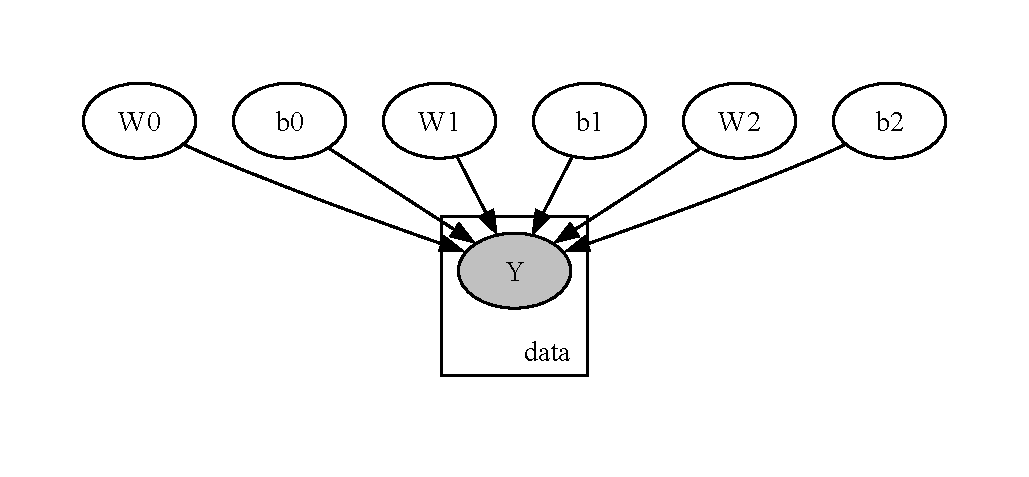
\includegraphics[width=0.7\textwidth]{plots/bnn_oscilator1_pinn.pdf}
    \caption{Graph of the general feed forward network}
    \label{fig:training_samples}
\end{figure}

\begin{figure}[h]
    \centering
    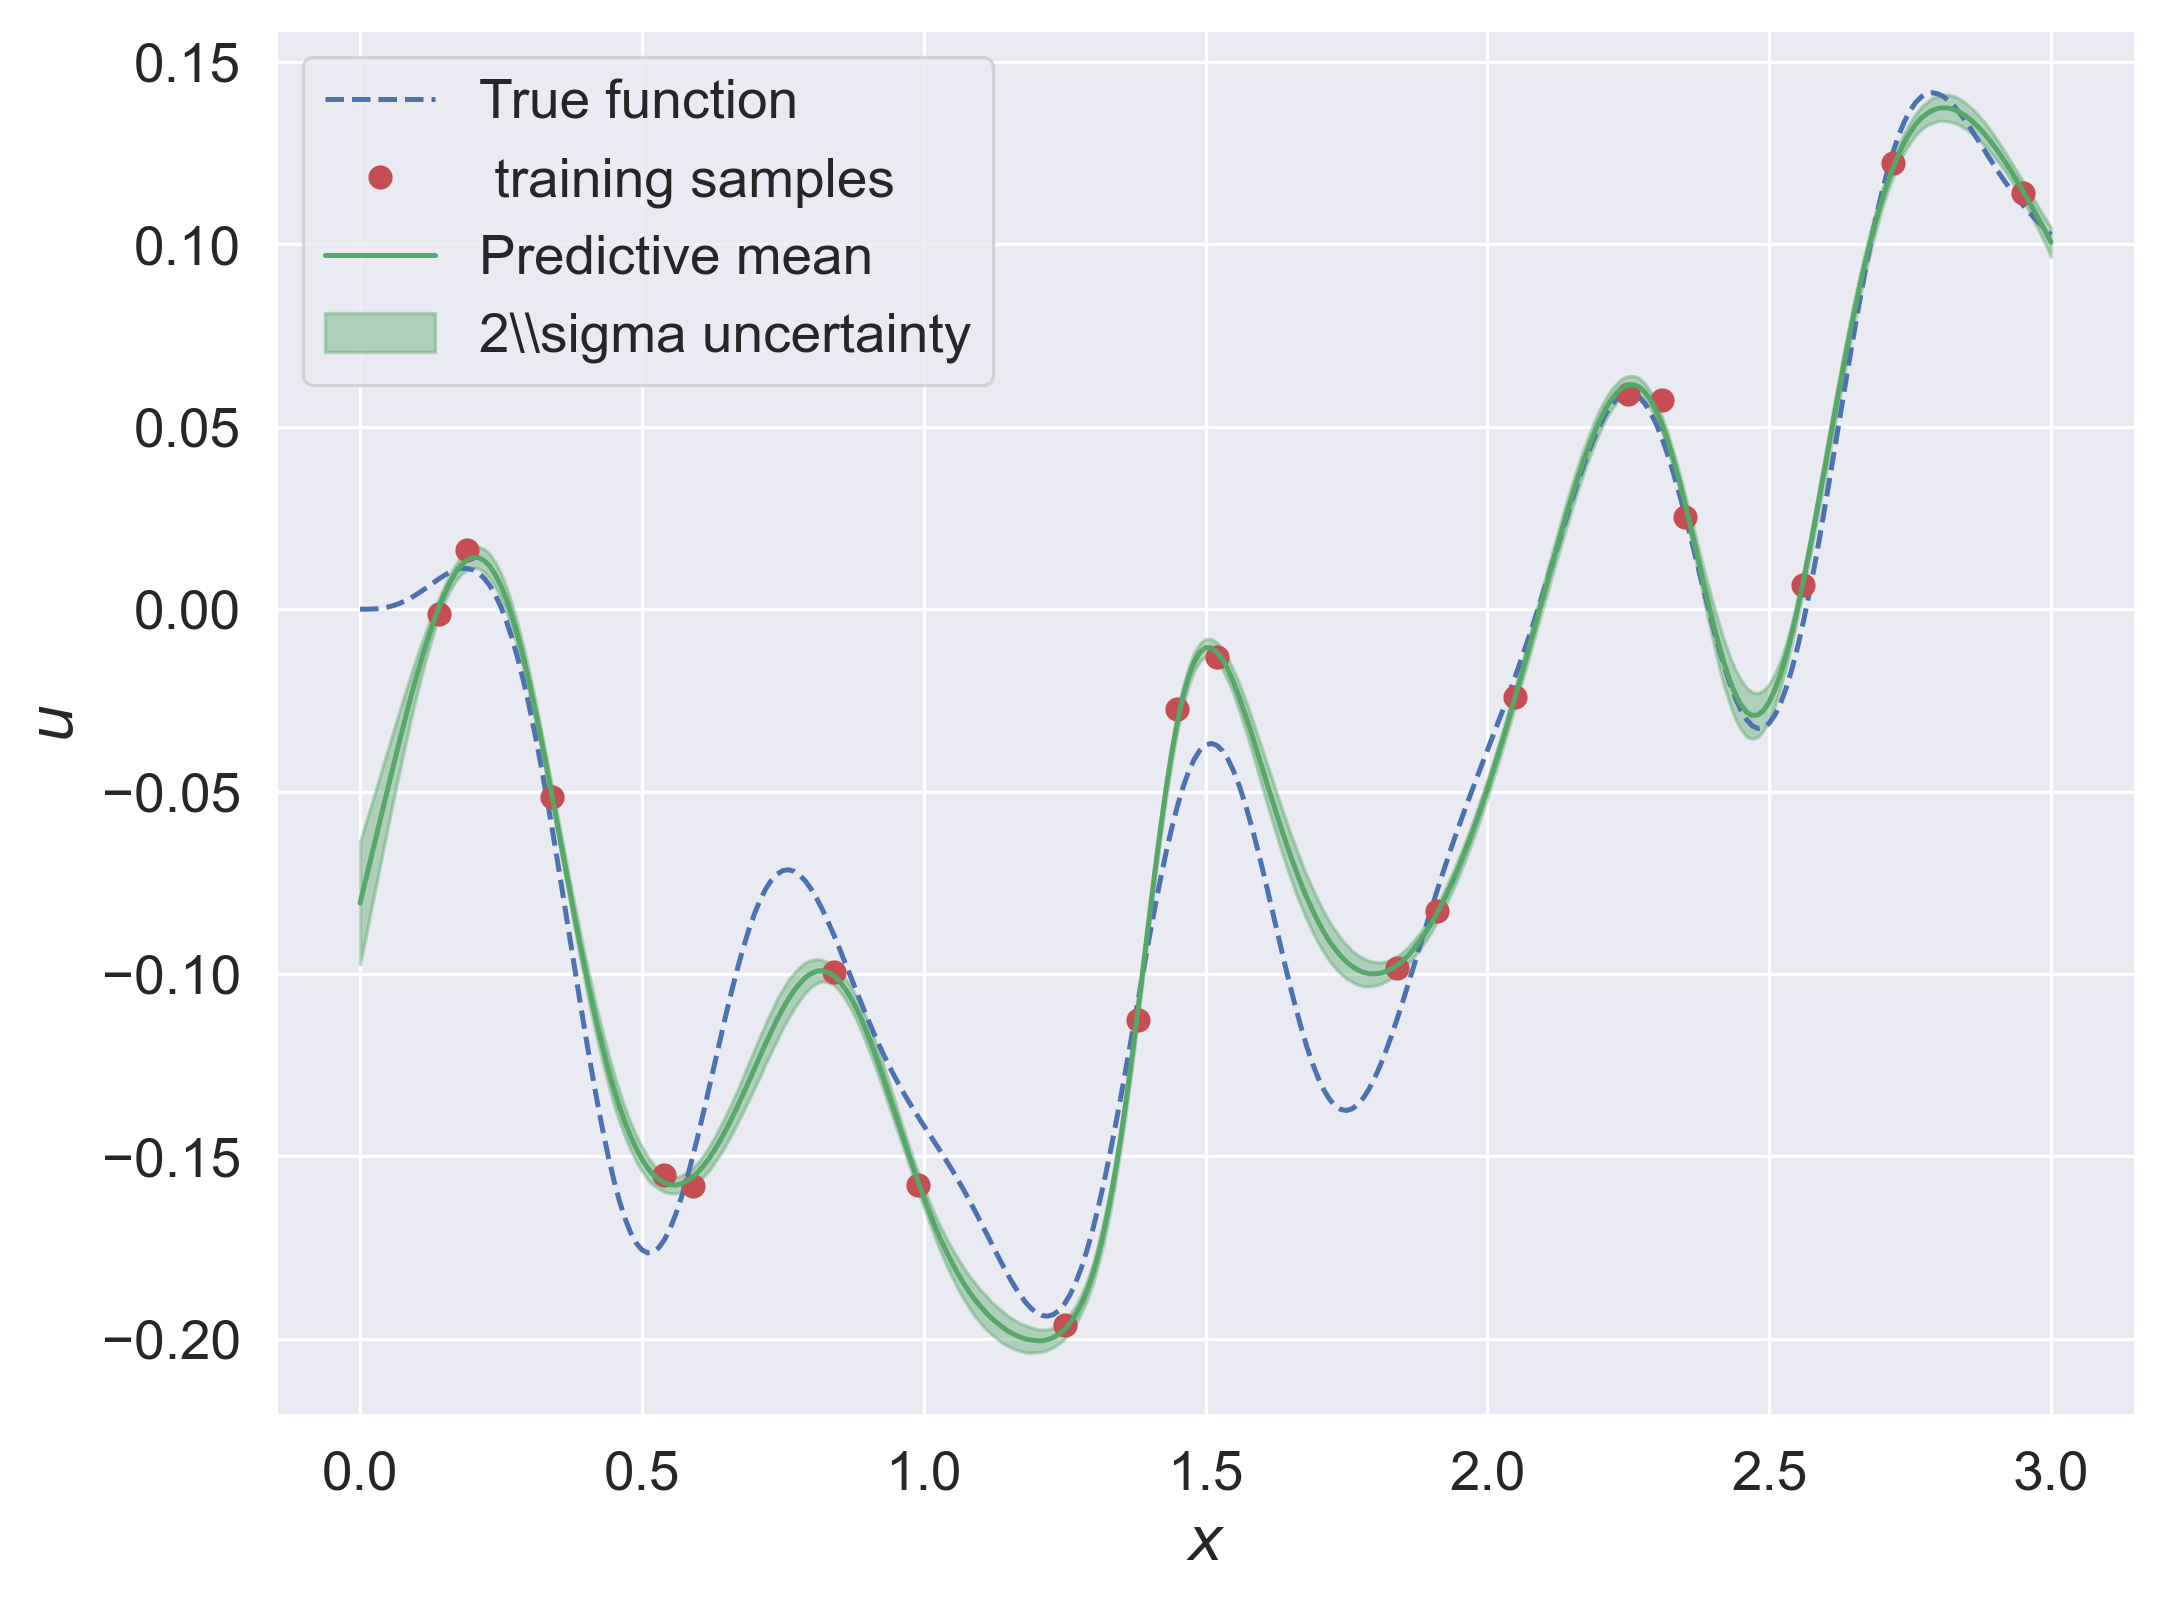
\includegraphics[width=0.6\textwidth]{plots/BNN/oscilator1_20_[20, 20, 1].png}
    \caption{ $n_\text{train}$ = 20  $rel \; L^2 = 0.09223274$}
    \label{fig:training_samples}
\end{figure}
\subsubsection{B-PINN}
For this example, also the data from the forcing term $f$ is used. Furthermore, the physical parameters \( m = 1 \), \( \gamma = 2 \), and \( k = 2 \) are introduced as probability distributions. They are assigned a prior and are then learned in the inference process. Again we show the properties of the model with the flowchart:
\begin{figure}[h]
    \centering
    \includegraphics[width=0.7\textwidth]{plots/BPINN/bnn_oscilator1_pinn.pdf}
    \caption{Graph of the physics informed BPINN model.}
    \label{fig:training_samples}
\end{figure}
Again a network with 2 hidden layers with 20 neurons is used, as well as the same 20 training points. The solution term $u$ and the forcing term $f$ can both, after the training stage, be predicted.
\begin{figure}[htbp!]
    \centering
    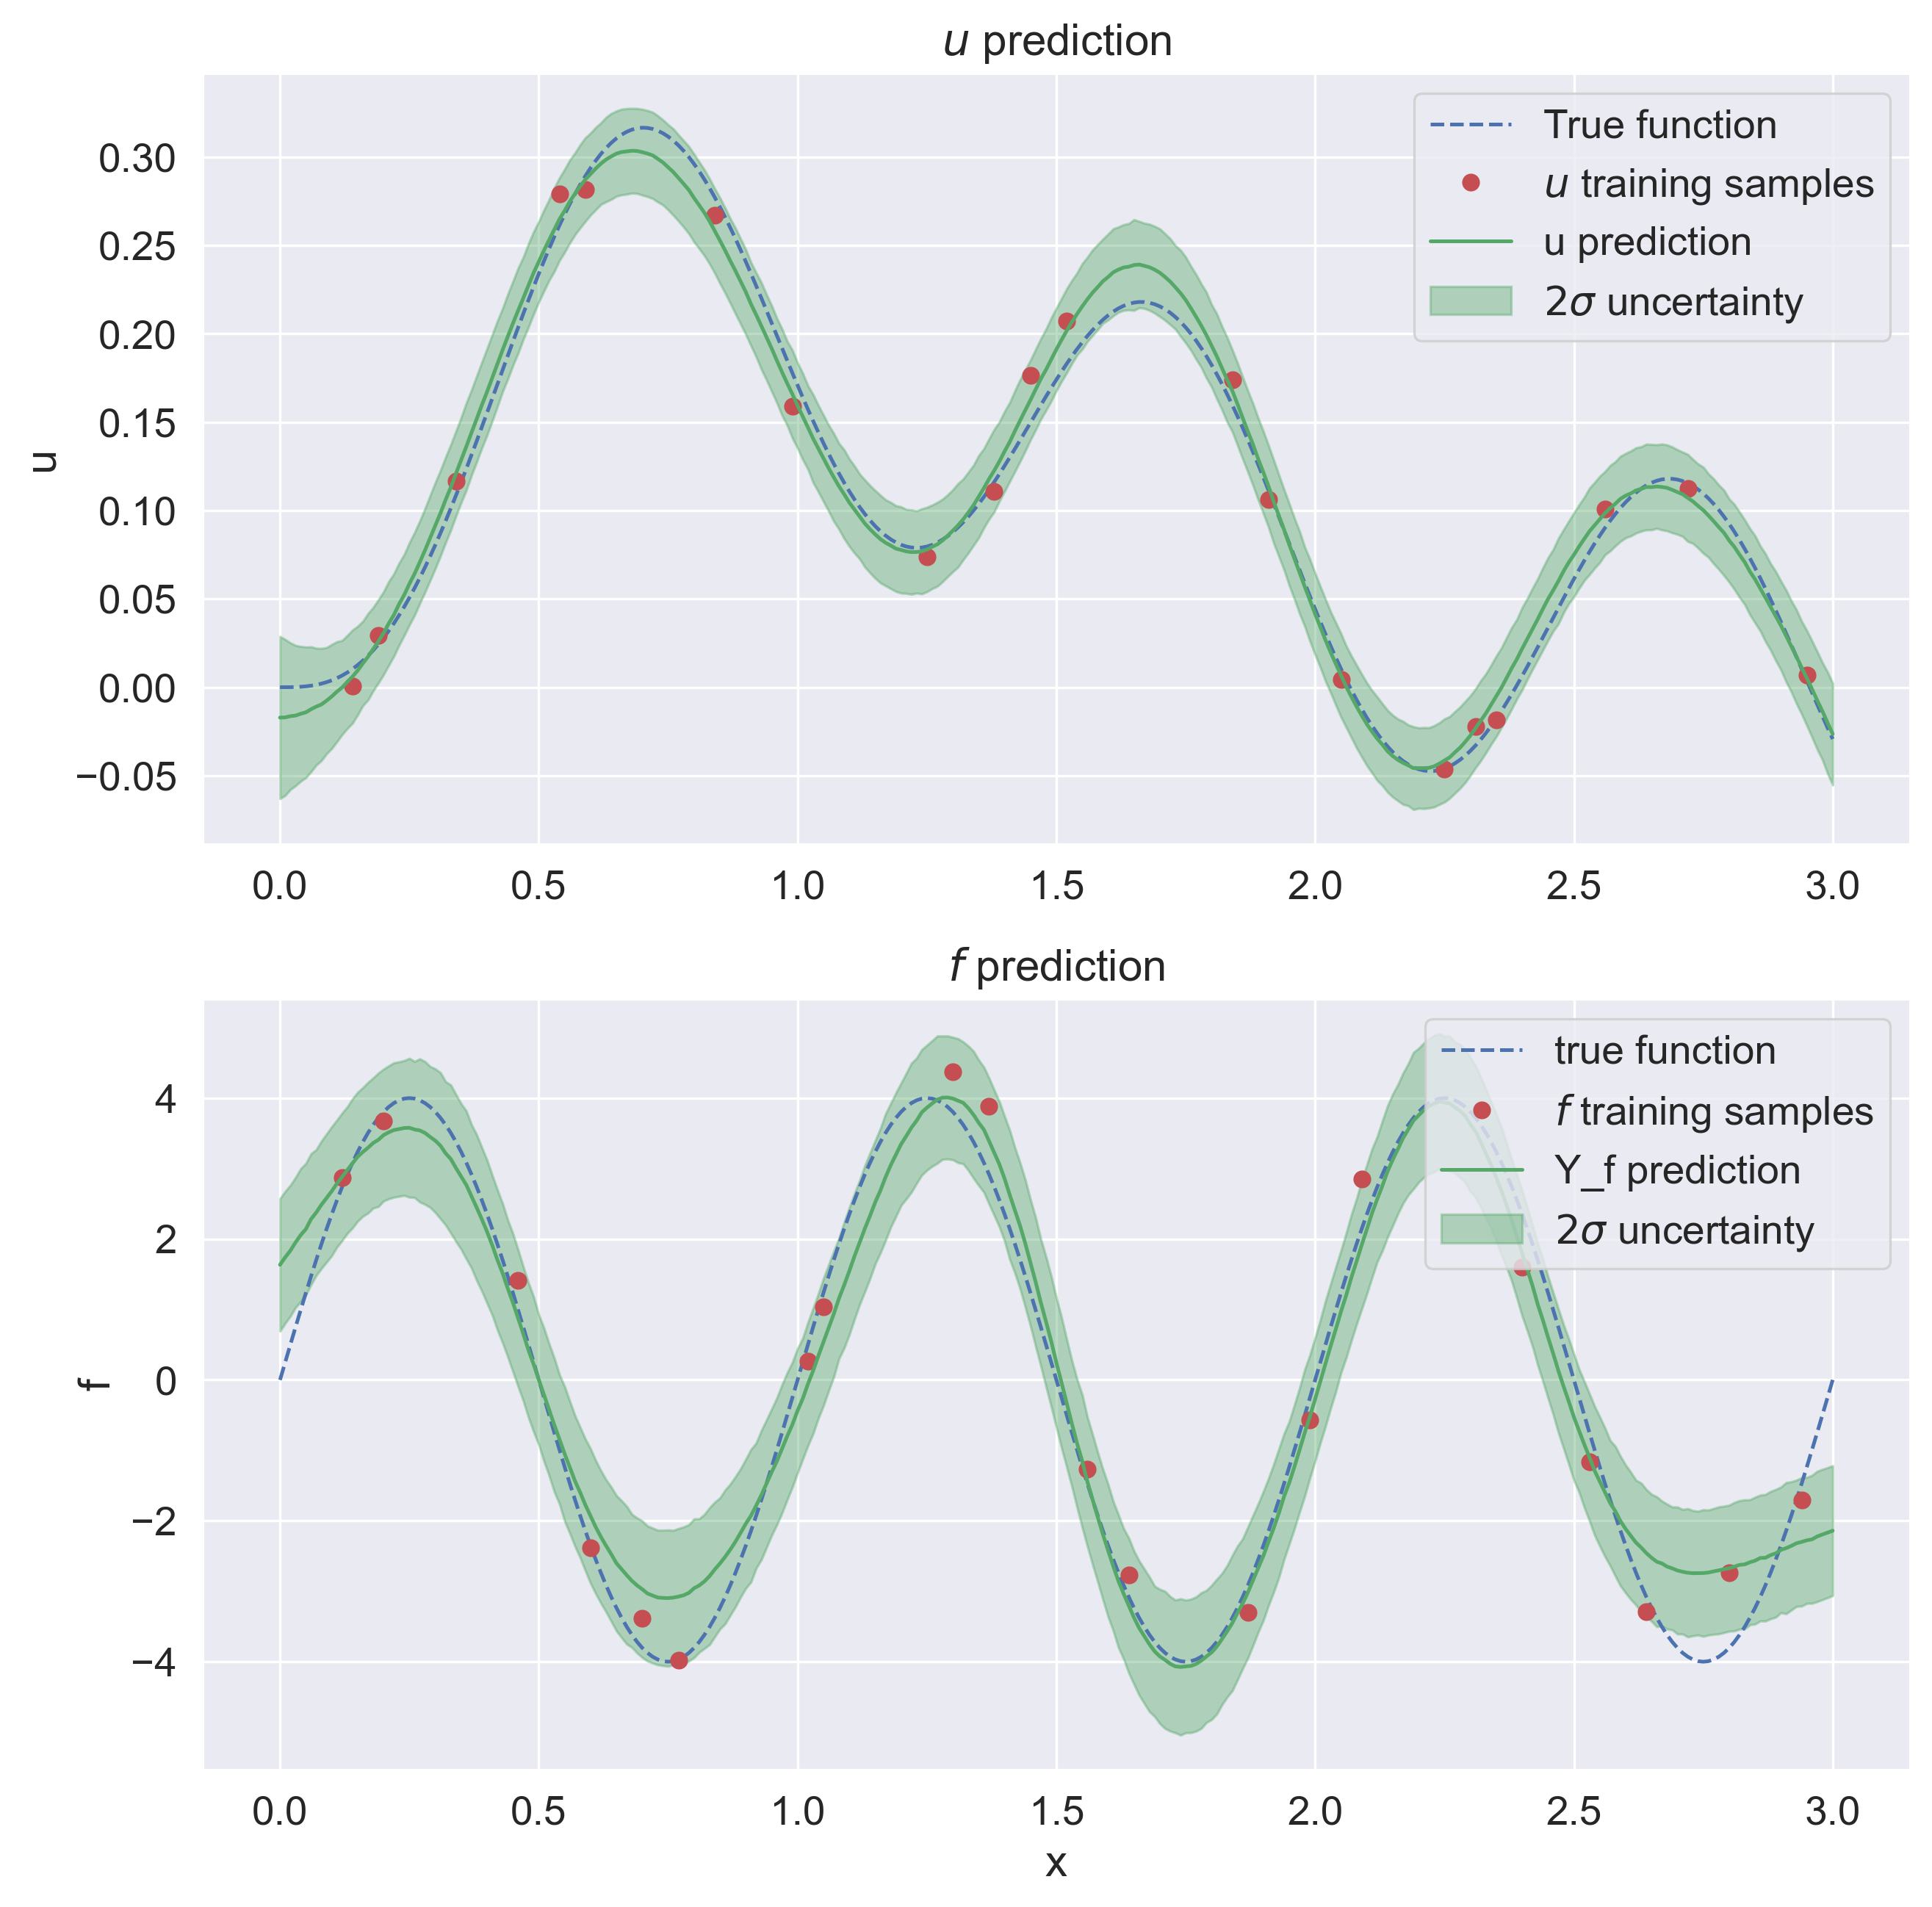
\includegraphics[width=0.6\textwidth]{plots/BPINN/oscilator1_20_[20, 20, 1].png}
    \caption{Samples from the training data for frequency domain relative L2 error relL2(u, u_hat):  0.07171381
relative L2 error relL2(f, f_hat):  0.2000248 0.01 0.4}
    \label{fig:training_samples}
\end{figure}
\begin{figure}[htbp!]
    \centering
    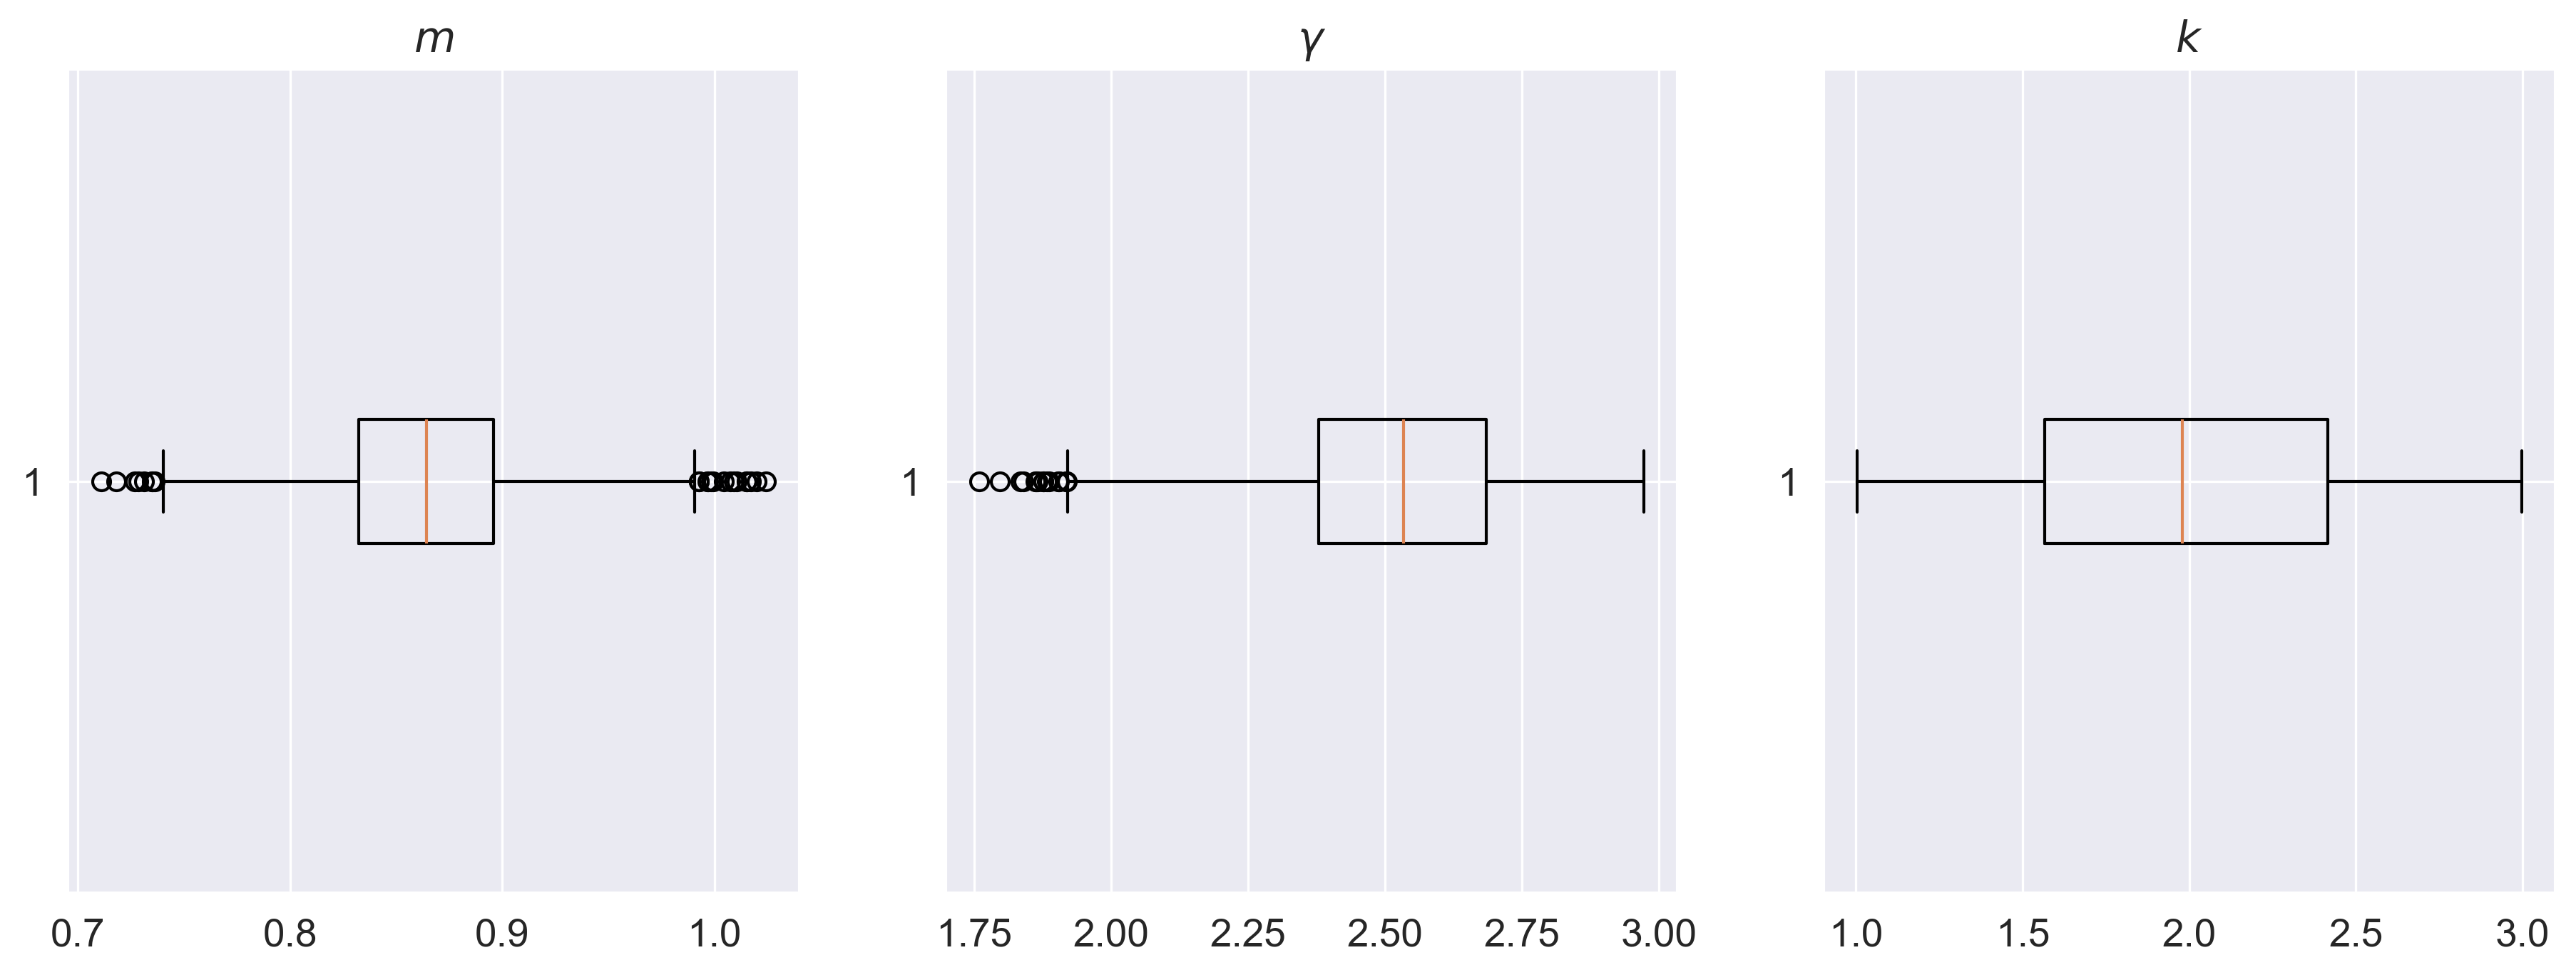
\includegraphics[width=0.6\textwidth]{plots/BPINN/params_oscilator1_20_[20, 20, 1].png}
    \caption{Samples from the training data for frequency domain}
    \label{fig:training_samples}
\end{figure}
Now we want to increase the amount of available training points and check the posterior distributions of the physical hyperparameters. 
\documentclass{article}
\usepackage{graphicx}
\usepackage{subcaption}

\begin{document}

\begin{figure}[htbp!]
    \centering
    % First row of plots
    \begin{subfigure}[b]{0.45\textwidth}
        \centering
        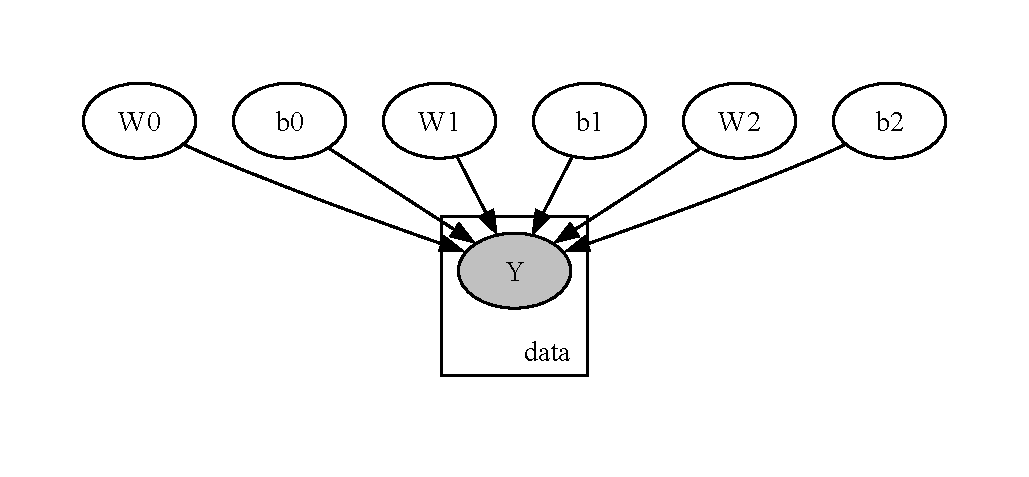
\includegraphics[width=\textwidth]{plots/bnn_oscilator1_pinn.pdf}
        \caption{Probability densities for the physical parameters \( m \), \( \gamma  \), and \( k \) with \nt=40}
        \label{fig:plot1}
    \end{subfigure}
    \hfill
    \begin{subfigure}[b]{0.45\textwidth}
        \centering
        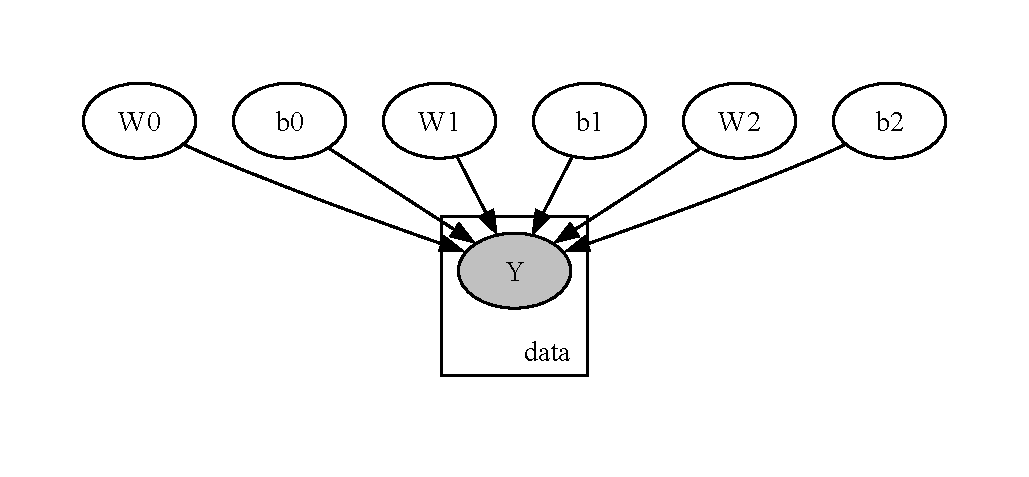
\includegraphics[width=\textwidth]{plots/bnn_oscilator1_pinn.pdf}
        \caption{Probability densities for the physical parameters \( m \), \( \gamma  \), and \( k \) with \nt=40}
        \label{fig:plot2}
    \end{subfigure}
    
    % Second row of plots
    \begin{subfigure}[b]{0.45\textwidth}
        \centering
        \includegraphics[width=\textwidth]{/bnn_oscilator1_pinn.pdf}
        \caption{Probability densities for the physical parameters \( m \), \( \gamma  \), and \( k \) with \nt=80}
        \label{fig:plot3}
    \end{subfigure}
    \hfill
    \begin{subfigure}[b]{0.45\textwidth}
        \centering
        \includegraphics[width=\textwidth]{/bnn_oscilator1_pinn.pdf}
        \caption{Probability densities for the physical parameters \( m \), \( \gamma  \), and \( k \) with \nt=80}
        \label{fig:plot4}
    \end{subfigure}
    
    \caption{Four plots arranged in two rows, two plots per row}
    \label{fig:four_plots}
\end{figure}

\end{document}


\newpage
\printbibliography
\newpage
\begin{appendices}
\section{Source Code}
\lstinputlisting[]{../code/network_functions.py}
\lstinputlisting[]{../code/oscillator.py}
\lstinputlisting[]{../code/B-PINN_oscillator.py}
\lstinputlisting[]{../code/utils.py}
\end{appendices}



\end{document}